** REMEMBER TEXT! **

\section{Pre-processing}

\subsection{Morphology} \label{sec:Morph}
The first representation of data is a binary matrix of the original pain maps. 
Firstly, the image of the original pain map is gray-scaled to get a one-dimensional matrix instead of a three-dimensional RGB-matrix. This matrix is then converted into a matrix consisting of zeroes and ones, where the pain areas are symbolized with ones. Afterwards the matrix is resized, since the given data has different sizes. Furthermore the matrix is cropped to sort out unnecessary data like the areas inferior and superior to the knee. An image consisting of a binary matrix is shown as figure \ref{fig:cropbin7}.

\begin{figure} [H]
\centering
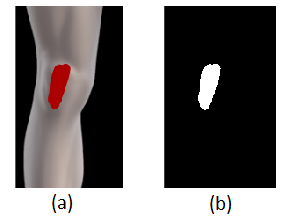
\includegraphics[width=0.3\textwidth]{figures/cropbin7}
\caption{Image consisting of a binary matrix where white color represents the pain.}
\label{fig:cropbin7}
\end{figure}

\noindent
To prepare the data for the first model all the binary matrices is converted into vectors, which are inserted into a new matrix with all images, where each row represent an image. The last value in each row represent the duration above (1) or below (0) XX value. REASON WHY!?

\subsection{Regions}
The second representation of the data is a matrix consisting of vectors with 20 values which indicate pain in relation to knee regions. 
The knee regions shown in figure ref{fig:atlas} is converted into a matrix consisting of 20 values, which represent the 20 knee regions. This matrix is superimposed to the binary image of the pain map, which results in a matrix with pain represented in each knee region. In figure \ref{fig:binregions} is there two illustrations of regions with different values (figure \ref{fig:binregions}(a) and the pain in the specific regions (figure \ref{fig:binregions}(b)).

\begin{figure} [H]
\centering
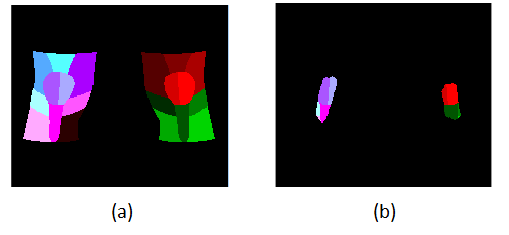
\includegraphics[width=0.8\textwidth]{figures/binregions}
\caption{(a) Knee regions and (b) pain in the specific regions.}
\label{fig:binregions}
\end{figure}

\noindent
After superimposing the two matrices, knee regions and pain, the number of pixels in each active knee region is found. This number is compared to the total number of pixels that are in each knee region, so a threshold is created to exclude the knee regions where there is less than 15 \% pain affected. WHY 15%. As an result is a vector with 20 values created, each value represent a knee region where pain above 15 % in the region is shown by ones and no pain as zeroes. 
Like in \ref{sec:Morph} all the vectors are inserted into a single matrix where each row represent an image. The last value represent the duration above (1) or below (0) XX value.


\subsection{Superimposed morphology and regions}
The third representation of the data is a matrix consisting of subjects pain divided into the knee regions.
\noindent
In this representation is the superimposed matrix from the second data representation used. Since the data representation should reflect the morphology of the pain and divide the pain into the different knee regions is one-hot encoding used. One-hot encoding is a way to separate categorical data into binary data \citep{Harris2012}. This means that the 20 values for each knee region do not have a correlation. After one-hot encoding the superimposed matrix consists of 20 layers where each layer represents a knee region.
As the other data representations is each matrix converted into a vector and inserted into a matrix with all the pain maps. The last column identify the duration above (1) or below (0) XX value. 
